\documentclass{article}
\usepackage{geometry}
\geometry{a4paper, margin=1in}
\usepackage{graphicx}
\usepackage[colorlinks=true, linkcolor=blue, citecolor=blue, urlcolor=blue]{hyperref}
\usepackage{listings}
\usepackage{xcolor}
\usepackage{amsmath}
\usepackage{enumitem}
\usepackage{float}

\lstset{
    language=NASM,
    basicstyle=\ttfamily\footnotesize\selectfont, % use the selected monospaced font
    backgroundcolor=\color{white},
    keywordstyle=\color{blue},
    commentstyle=\color{gray},
    stringstyle=\color{red},
    numbers=left,
    numberstyle=\tiny\color{gray},
    stepnumber=1,
    numbersep=10pt,
    frame=single,
    breaklines=true,
    captionpos=b,
    tabsize=4
}

\title{Assignment 1: v01 - Booting and Logo in One Sector}
\author{
    [Welby Seely] \\
    \texttt{[wseely@emich.edu]}
}
\date{\today}

\begin{document}

    \maketitle
    \section{Intro}\label{sec:intro}
    A simple program was implemented to serve as the ``splash screen'' of the bootloader of a custom
    operating system.

    The program uses VGA graphics mode with 320 x 200 resolution and 256 colors to display a
    custom `W' logo and the required text for the splash screen.

    After entering any key, the program switches to text mode and display a magenta `\$' and a
    blinking cursor.

    This fulfills the basic requirements:

    \begin{itemize}
        \item When booted, it displays a welcome message.
        \item It waits for a key stoke.
        \item After key stoke, the welcome is cleared.
        \item Then a command prompt `\$' at the top left corner followed by a blinking cursor.
    \end{itemize}

    \section{Welcome Message Requirements}\label{sec:reqs}
    The more detailed requirements have been fulfilled as well:

    \begin{itemize}
        \item String of your OS name, your name, the OS version, current version.
            \begin{itemize}
                \item OS name: WelbOS
                \item Name: Welby Seely
                \item OS' current version: v01
            \end{itemize}
        \item A creative OS logo
            \begin{itemize}
                \item This was difficult given the 512 byte constraint.
                I designed a 16 x 9 bitmap of a `W' to act as the logo to minimize the amount of space the logo takes.
                \item This logo is drawn and scaled by a factor of 8 - this scalar is customizable as a constant, and could be easily parameterized.
                \item I wanted something more interesting than a monochrome letter, so I added a red gradient.
                This would be easy if using something like true 16-bit color, but VGA can only display 256 colors at a time, so only two shades of red are available by default.
                I got around this by programming the DAC (Digital to Analog Converter).
                BIOS provides output ports to override the default palette, the assignment of 6-bit RGB colors to the 256 indices.
                I reprogrammed arbitrary indices to represent a sliding intensity of red for each of the 9 logo rows.
            \end{itemize}
        \item Double lined borders such as C8h, C9h
            \begin{itemize}
                \item \textit{C9h, CDh, BBh, C8h, and BCh} were used for creating borders in addition to the logo.
            \end{itemize}
        \item At least 5 different colors
            \begin{itemize}
                \item 9 different colors were used for the logo (shades of red), red was used for the text and block characters, gold for the ``Press any key\ldots'' message, and magenta for the `\$' prompt.
            \end{itemize}
        \item Block characters such as B0h, DCh
            \begin{itemize}
                \item \textit{DE, DC, and DD} were used as block characters.
            \end{itemize}
        \item Loops are required to display long horizontal borders.
            \begin{itemize}
                \item Loops were used to display the horizontal borders in the \textit{draw\_row} procedure.
            \end{itemize}
        \item Message to indicate that using a key press to continue
            \begin{itemize}
                \item ``Press any key to continue\ldots'' was implemented in yellow.
            \end{itemize}
        \item Graphical mode in BIOS is optional but will be evaluated highly.
        \begin{itemize}
            \item Graphical mode was used for rendering, scaling, and displaying the logo/splash screen.
        \end{itemize}
    \end{itemize}

    \section{Screenshots}\label{sec:screenshots}
    Screenshots of the splash screen and the prompt screen are provided.

    \begin{figure}[H]  % [H] forces the figure to appear here
        \centering
        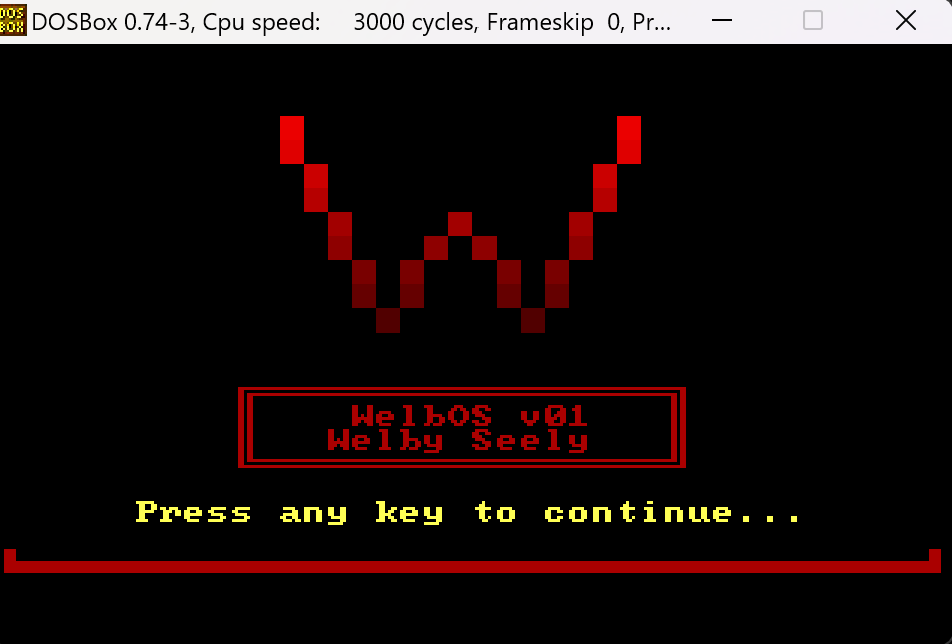
\includegraphics[width=\textwidth]{splash-screen} % Scales image to document width
        \caption{Custom splash screen, complete with logo in graphics mode}
        \label{fig:1}
    \end{figure}

    \begin{figure}[H]  % Ensures figure appears right here
        \centering
        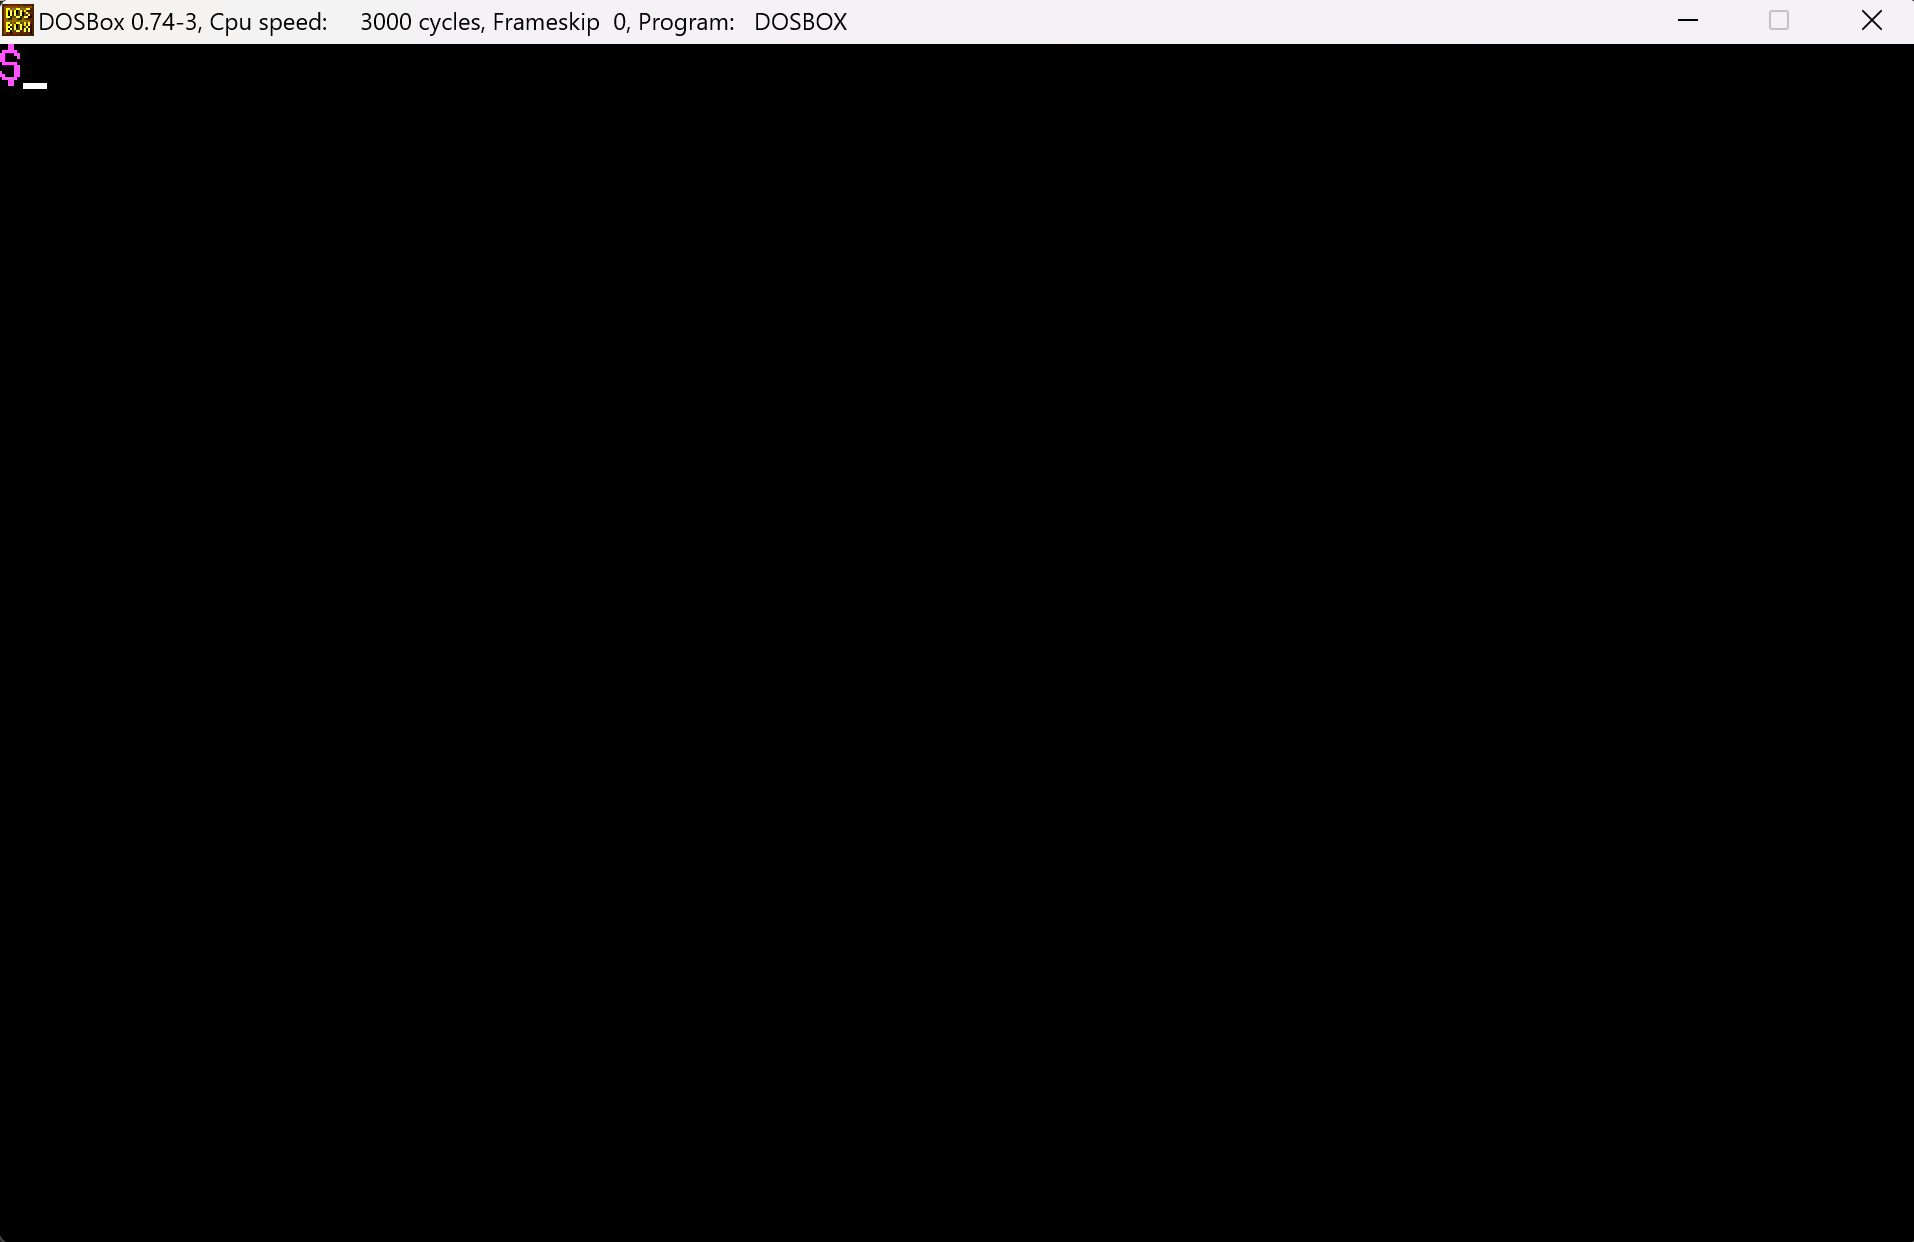
\includegraphics[width=\textwidth]{prompt} % Scales image to document width
        \caption{Prompt with \$ and a blinking cursor}
        \label{fig:2}
    \end{figure}

    \section{Appendix 1: Source Code}\label{sec:appendix_1}
    \begin{lstlisting}
        bits 16
        VIDEO_SERVICES      equ 0x10
        FUN_DISPLAY         equ 0x13
        FUN_VIDEO_MODE      equ 0x0000
        VGA_MODE            equ 0x0013
        TEXT_MODE           equ 0x0003
        FUN_CURSOR_POS      equ 0x02

        KEYBOARD_SERVICES   equ 0x16
        TERMINATE_PROGRAM   equ 0x20

        VGA_DISPLAY_WIDTH   equ 320
        DISPLAY_WIDTH       equ 80
        DISPLAY_HEIGHT      equ 25
        VGA_TXT_DISP_WIDTH  equ 40
        VGA_TXT_DISP_HEIGHT equ 25
        MESSAGE_ROW         equ VGA_TXT_DISP_HEIGHT / 2 + 3
        LINE_ROW_TOP        equ MESSAGE_ROW - 1
        LINE_ROW_NAME       equ MESSAGE_ROW + 1
        LINE_ROW_BOTTOM     equ LINE_ROW_NAME + 1
        LINE_ROW_ANYKEY     equ LINE_ROW_BOTTOM + 2
        TEXT_MODE           equ 0x03
        MAGENTA_BLACK       equ 0x0D
        WHITE_BLACK         equ 0x0F
        RED_BLACK           equ 0x04
        YELLOW_BLACK        equ 0x0E
        LIGHT_RED           equ 0x0C
        LOGO_START_X        equ (VGA_DISPLAY_WIDTH - (16 * SCALING_FACTOR)) / 2
        LOGO_START_Y        equ (200 - (9 * SCALING_FACTOR)) / 2 -40

        SCALING_FACTOR      equ 0x8
        FALSE               equ 0x00


        %define CENTER_TXT(len) ((DISPLAY_WIDTH - len) / 2)
        %define CENTER_VGA_TXT(len) ((VGA_TXT_DISP_WIDTH - len) / 2)

        org 0x7c00
        jmp short start
        nop

        bsOEM       db "WelbOS v01"           ; OEM String

        start:
            mov ax, FUN_VIDEO_MODE + VGA_MODE ; Dim: 320 x 200 in pixels, 40 x 25 in text characters
            int VIDEO_SERVICES

            call set_red_gradient_palette
            call draw_logo

            push RED_BLACK
            push welboslen
            push welbos
            push MESSAGE_ROW
            push CENTER_VGA_TXT(welboslen)
            call print

            push RED_BLACK
            push welboslen - 1               ; Repeat count
            push CENTER_VGA_TXT(welboslen)   ; Column
            push LINE_ROW_TOP                ; Row
            push topline                     ; Address of 3-tuple
            call draw_line

            push RED_BLACK
            push namelen
            push name
            push LINE_ROW_NAME
            push CENTER_VGA_TXT(namelen)
            call print

            push RED_BLACK
            push welboslen - 1                ; Repeat count
            push CENTER_VGA_TXT(welboslen)    ; Column
            push LINE_ROW_BOTTOM              ; Row
            push bottomline                   ; Address of 3-tuple
            call draw_line

            push YELLOW_BLACK
            push anykeylen
            push anykey
            push LINE_ROW_ANYKEY
            push CENTER_VGA_TXT(anykeylen)
            call print

            push RED_BLACK
            push VGA_TXT_DISP_WIDTH - 1       ; Repeat count
            push 0                            ; Column
            push LINE_ROW_ANYKEY + 2          ; Row
            push blockline                    ; Address of 3-tuple
            call draw_line

            ; Wait for key press
            mov ah, 0x00
            int KEYBOARD_SERVICES

            ; Switch back to text mode (80x25)
            mov ax, TEXT_MODE
            int VIDEO_SERVICES

            call clear_screen
            call reset_cursor_pos

            push MAGENTA_BLACK
            push 1
            push prompt_sym
            push 0
            push 0
            call print
        end:
            int TERMINATE_PROGRAM

        ; -----------------------------------------------------------------------------
        ; Procedure: draw_logo
        ; Description: Draws the bootloader logo to the screen.
        ; Inputs: None. TODO - X and Y coordinates
        ; Outputs: None.
        ; Modifies:
        ;   - AX, BX, BL, DI, ES, SI
        ;   - Segment 0xA000 (BIOS memory mapped VHA region)
        ; Calls: N/A
        ; Notes: Assumes BIOS is in VGA mode
        ; -----------------------------------------------------------------------------
        draw_logo:
            mov ax, 0xA000     ; memory mapped I/O segment for VGA
            mov es, ax

            mov di, LOGO_START_Y * VGA_DISPLAY_WIDTH + LOGO_START_X
            mov si, w_bitmap           ; source bitmap start address

            mov dx, 9                  ; logical row that we're calculating
            push SCALING_FACTOR

        .draw_rows:
            mov bx, 9
            sub bx, dx                 ; determine color for this row
            mov bl, [row_colors + bx]  ; store row color in BL
            mov ax, [si]               ; retrieve pixels for this row

            mov cx, 16                 ; Process 16 pixels
        .draw_row:
            shl ax, 1                  ; Shift left (test MSB of AX)
            jnc .skip_column

            push cx
            push ax
            mov cx, SCALING_FACTOR
            mov al, bl
            rep stosb
            pop ax
            pop cx
            jmp .next_column
        .skip_column:
            add di, SCALING_FACTOR
        .next_column:
            loop .draw_row

        .scale_vertically:
            add di, 320 - 16 * SCALING_FACTOR ; Move to next VGA row
            pop cx
            dec cx
            cmp cx, 0
            jz .next_source_row
            push cx
            jmp .draw_rows
        .next_source_row:
            add si, 2
            dec dx
            jz .logo_done
            push SCALING_FACTOR
            jmp .draw_rows
        .logo_done:
            ret

        ; -----------------------------------------------------------------------------
        ; Procedure: draw_line
        ; Description: Draws a line for the splash screen in both text and graphics modes.
        ; Inputs:
        ;   - [sp+4] Address of 3-tuple of ASCII characters
        ;   - [sp+6] Row
        ;   - [sp+8] Column
        ;   - [sp+10] Number of times to repeat line body
        ;   - [sp+12] Color of the string.
        ; Modifies:
        ;   - AX, BX, BL, DI, ES, SI
        ; Calls: print
        ; -----------------------------------------------------------------------------
        draw_line:
            push bp
            mov bp, sp

            ;left edge
            push word [bp + 12]
            push 1
            mov si, [bp + 4]
            push si
            mov si, [bp + 6]
            push si
            mov si, [bp + 8]
            push si
            call print

            ; set up middle loop
            mov ax, 1                           ; break when == to cx
        .draw_line_middle:
            mov cx, [bp + 10]
            cmp ax, cx
            je .draw_line_right
            push ax

            push word [bp + 12]
            push 1
            mov si, [bp + 4]
            inc si
            push si
            mov si, [bp + 6]
            push si
            mov si, [bp + 8]
            add si, ax
            push si
            call print

            pop ax
            inc ax
            jmp .draw_line_middle

        .draw_line_right:
            push word [bp + 12]
            push 1
            mov si, [bp + 4]
            add si, 2
            push si
            mov si, [bp + 6]
            push si
            add ax, [bp + 8]                    ; rightmost position
            push ax
            call print

            pop bp
            ret 10

        ; -----------------------------------------------------------------------------
        ; Procedure: reset_cursor_pos
        ; Description: Resets curor position to top left
        ; Inputs: None.
        ; Outputs: None.
        ; Modifies:
        ;   - ah, bh, dh, dl
        ; Calls:
        ;   - VIDEO_SERVICES (0x10)
        ; -----------------------------------------------------------------------------
        reset_cursor_pos:
            mov ah, FUN_CURSOR_POS       ; BIOS Procedure: set cursor position
            mov bh, 0x00                 ; Page number (0)
            mov dh, 0x00                 ; Row (0)
            mov dl, 0x01                 ; Column (1)
            int VIDEO_SERVICES
            ret

        ; -----------------------------------------------------------------------------
        ; Procedure: set_red_gradient_palette
        ; Description: Sets gradient for the logo
        ; Inputs: None.
        ; Outputs: None.
        ; Modifies:
        ;   - No registers
        ;   - port 0x3C8, VGA color index port
        ;   - port 0x3C9, VHA RGB color data port
        ; Calls:
        ;   - N/A
        ; -----------------------------------------------------------------------------
        set_red_gradient_palette:
            mov dx, 0x3C8   ; VGA color index port - this will be incremented after writing an RGB triplet
            mov al, 32      ; Start setting colors from palette index 32
            out dx, al
            inc dx          ; Set dx = 0x3C9 (RGB color data port to write triplet to)

            mov cx, 9       ; 9 shades for 9 rows of the "W"
            mov si, red_shades
        .next_color:
            mov al, [si]    ; Load color intensity
            out dx, al      ; Set R
            xor al, al      ; Set G=0
            out dx, al
            out dx, al      ; Set Blue=0
            inc si
            loop .next_color
            ret

        ; -----------------------------------------------------------------------------
        ; Procedure: clear_screen
        ; Description: Clears and resets the screen in text mode.
        ; Inputs: None.
        ; Outputs: None.
        ; Modifies:
        ;   - AX, BX, CX, DX
        ; Calls:
        ;   - BIOS interrupt 0x10, Procedure 0x06.
        ; -----------------------------------------------------------------------------
        clear_screen:
            mov ah, 0x06            ; BIOS scroll (Procedure 06h)
            mov al, 0               ; Scroll all lines
            mov bh, WHITE_BLACK         ; Attribute
            mov ch, 0               ; Upper-left row
            mov cl, 0               ; Upper-left column
            mov dh, 24              ; Lower-right row
            mov dl, 79              ; Lower-right column
            int VIDEO_SERVICES          ; BIOS video interrupt
            ret

        ; -----------------------------------------------------------------------------
        ; Procedure: print
        ; Description: Prints a string to the console.
        ; Inputs:
        ;   - [sp+4] Column position to begin writing the string.
        ;   - [sp+6] Row position to begin writing the string.
        ;   - [sp+8] Memory address location of the string.
        ;   - [sp+10] Length of the string.
        ;   - [sp+10] Color of the string.
        ; Outputs: None.
        ; Modifies:
        ;   - AX, BX, CX, DX
        ; Calls:
        ;   - BIOS interrupt 0x10, Procedure 0x13.
        ; -----------------------------------------------------------------------------
        print:
            push bp ; save bp for the return
            mov  bp, sp ; update bp to create a new "stack frame"

            mov bl, [bp+12]        ; Attribute (lightgreen on black)
            mov cx, [bp+10]        ; length of the string
            mov si, [bp+8]         ; address of the string
            mov dh, [bp+6]         ; row position
            mov dl, [bp+4]         ; column position

            ; We need ES:BP provides the pointer to the string - load the data segment (DS) base into ES
            push ds
            pop es

            mov  ah, FUN_DISPLAY    ; BIOS display string (Procedure 13h)
            mov  al, 0              ; Write mode = 1 (cursor stays after last char
            mov  bh, 0              ; Video page
            mov  bp, si             ; Put offset in BP (ES:BP points to the string)
            int  VIDEO_SERVICES

            pop bp                 ; Restore stack frame
            ret 10

        ; data:
        topline             db 0xC9
                            db 0xCD
                            db 0xBB
        bottomline          db 0xC8
                            db 0xCD
                            db 0xBC
        blockline           db 0xDE
                            db 0xDC
                            db 0xDD
        welbos              db 0xBA, `    WelbOS v01   `, 0xBA
        welboslen           equ ($ - welbos)
        name                db 0xBA, `   Welby Seely   `, 0xBA
        namelen             equ ($ - name)
        anykey              db "Press any key to continue..."
        anykeylen           equ ($ - anykey)
        prompt_sym          db "$"
        w_bitmap db 02h, 80h
                 db 02h, 80h
                 db 04h, 40h
                 db 04h, 40h
                 db 08h, 21h
                 db 88h, 22h
                 db 50h, 14h
                 db 50h, 14h
                 db 20h, 08h
        red_shades db 58, 55, 50, 45, 40, 35, 30, 25, 20; Bright to dark red
        ; Row color table, from top to bottom row
        row_colors db 32, 33, 34, 35, 36, 37, 38, 39, 40  ; Use only custom red shades
        ; Pad to 512 bytes for an MBR:
        padding times 510 - ($ - $$) db 0

        ; Optional boot signature:
        bootSig db 0x55, 0xAA
    \end{lstlisting}

\end{document}
